%        File: CurveRepulsion1.tex
%     Created: Fri Jan 20 05:00 PM 2023 G
% Last Change: Fri Jan 20 05:00 PM 2023 G
%
\documentclass[a4paper, 11pt]{article}

\usepackage[]{amsmath}
\usepackage{amssymb}
\usepackage{mathtools}
\usepackage{amsthm}
\usepackage{graphicx}
\graphicspath{ {./images/} }

\newcommand{\x}{\mathbf{x}}
\newcommand{\dx}{\,\text{d}x}
\newcommand{\dy}{\,\text{d}y}
\newcommand{\norm}[1]{||#1||}
\newcommand{\inner}[1]{\langle \langle #1 \rangle \rangle}

\DeclareMathOperator{\grad}{grad}
\DeclareMathOperator{\Var}{Var}

\theoremstyle{definition}
\newtheorem{definition}{Definition}
\theoremstyle{remark}
\newtheorem{remark}{Remark}


\title{Curve Repulsion - 1}
\date{20/01/2023}
\author{Paul Kim}

\begin{document}
\maketitle

\section{Theory behind Discretization}
\begin{figure}[h]
    \centering
    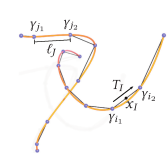
\includegraphics[scale=0.5]{discretization.png}
    \caption{Discretization process}
\end{figure}
We now consider a discretization of a curve.
Index the points on the curve by $\mathcal{I} = \left\{ 1, 2, \cdots,  J \right\}$, such that
points are given by $\left\{ \gamma_1, \gamma_2, \cdots, \gamma_J \right\}$

Using the similar notation to the paper by Yu, Schumacher, and Crane,
for edge $I = \left\{ \gamma_i, \gamma_j \right\} \in E$
and for function $u: \mathbb{R}^3 \rightarrow \mathbb{R}$
\begin{itemize}
    \item $l_I \coloneqq | \gamma_i - \gamma_j |$
    \item $T_I \coloneqq \frac{\gamma_j - \gamma_i}{l_I}$
    \item $\x_I \coloneqq \frac{\gamma_i + \gamma_j}{2}$
    \item $u_I \coloneqq \frac{u_i + u_j}{2}$
        \begin{itemize}
            \item Syntactic sugar: $u_i \equiv u\left( \gamma_i \right)$
        \end{itemize}
    \item $u[I] \coloneqq 
        \begin{pmatrix}
            u_i \\
            u_j
        \end{pmatrix}
        $
\end{itemize}

\subsection{Discrete Energy}
The na\"ive discretization of $\mathcal{E}_{\beta}^\alpha \coloneqq \iint_{M^2} k_{\beta}^{\alpha} \left( \gamma \left( x \right), \gamma \left( y \right), T\left( x \right) \right) \dx_{\gamma} \dy_{\gamma}$
where $k_{\beta}^{\alpha} \left( p, q, T \right) \coloneqq \frac{|T \times \left( p-q \right)|^\alpha}{|p-q|^{\beta}}$
is given by
\begin{equation}
    \sum_{I \in E} \sum_{J \in E} \int_{\bar I} \int_{\bar J} k_{\beta}^{\alpha} \left( \gamma (x), \gamma (y), T_I \right) \dx_{\gamma} \dy_{\gamma}
    \label{equ: Ill-defined Discrete Energy}
\end{equation}
However, in a polygonal curve (hence the discretized curve), (\ref{equ: Ill-defined Discrete Energy}) is ill-defined.
\begin{figure}[h]
    \centering
    
\includegraphics[scale=0.5]{polygon.png}
    \caption{Near each vertex, the integrand is unbounded.}
\end{figure}

So resolve this by removing the two neighboring edges.\footnote{In the limit, the contribution from this
removed edge goes to zero.}
Also approximate the kernel by the average of the kernel evaluated at each pair of appropriate edges (total: 4)
\begin{align}
    \hat{\mathcal{E}}_{\beta}^{\alpha} &\coloneqq \sum_{I, J \in E, I \cap J = \emptyset} \left( \hat{k}_{\beta}^\alpha \right)_{I,J} l_I l_J \\
    \left( \hat{k}_{\beta}^{\alpha} \right)_{I,J} &\coloneqq \frac{1}{4} \sum_{i \in J, j \in J} k_{\beta}^{\alpha} \left( \gamma_i, \gamma_j, T_I \right)
\end{align}

\section{Discrete Gradient Flow in $L^2$ for Closed Loop}
Suppose a curve is discretized as position vectors:
$x_1, x_2, \cdots, x_J$ (and $x_{J+1} \coloneqq x_1$).

Also denote the edge from $x_i$ to $x_{i+1}$ as $I_i$ (as opposed to the previous section).

The \textbf{discretized energy} $E$ can be expressed as:
\begin{align}
    E &= \sum_{i = 1}^{J} \sum_{\substack{j = 1 \\ |j-i| > 1}} k_{i,j} \norm{x_{i+1} - x_i} \, \norm{x_{j+1} - x_j} 
    \label{equ: Discretized Energy}
    \\
    k_{i,j} &= \frac{1}{4} \left( 
        k_{\beta}^{\alpha} \left( x_i, x_j, T_i \right)
        + k_{\beta}^{\alpha} \left( x_i, x_{j+1}, T_i \right)
        + k_{\beta}^{\alpha} \left( x_{i+1}, x_j, T_i \right)
        + k_{\beta}^{\alpha} \left( x_{i+1}, x_{j+1}, T_i \right)
    \right)
\end{align}

\begin{figure}[h]
    \centering
    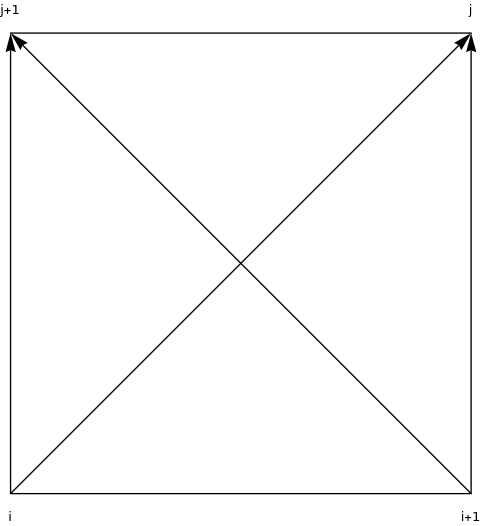
\includegraphics[scale=0.6]{kernel-2x2.png}
    \caption{Kernel $k_{i,j}$ computation}
\end{figure}

Recall the definition of differential, gradient, and gradient flow.
\begin{definition}[Differential]
    Given functional $\mathcal{E}(\gamma)$, the \textbf{differential} is defined as:
    \begin{equation}
        \text{d}\mathcal{E}|_{\gamma} (u) = \lim_{\epsilon \rightarrow 0} \frac{1}{\epsilon} \left( \mathcal{E}\left( \gamma + \epsilon u \right) - \mathcal{E}\left( \gamma \right) \right)
    \end{equation}
\end{definition}

\begin{definition}[Gradient]
    Given functional $\mathcal{E}\left( \gamma \right)$ and space $V$, the \textbf{gradient} $\grad \mathcal{E}$ is the unique function satisfying the following for any function $u$:
    \begin{equation}
        \inner{\grad \mathcal{E}, u}_V = \text{d} \mathcal{E} (u)
    \end{equation}
    Note that the LHS is a inner product of two vector-valued functions.
    A natural inner product in $L^2$ to define is:
    \begin{equation}
        \inner{u,v}_{L^2} \coloneqq \int_{\Omega} u \cdot v \dx
    \end{equation}

\end{definition}

\begin{definition}[Gradient Flow]
    Given functional $\mathcal{E}(\gamma)$, the \textbf{gradient flow} equation is defined as:
    \begin{equation}
        \frac{d}{dt} \gamma = - \grad \mathcal{E} (\gamma)
    \end{equation}
    Note that $\gamma = \left( \gamma_x, \gamma_y, \gamma_z \right)^T \in \mathbb{R}^3$, so it might be clearer to write:
    \begin{equation}
        \frac{d}{dt}
        \begin{pmatrix}
            \gamma_x \\
            \gamma_y \\
            \gamma_z
        \end{pmatrix}
        =
        \grad \mathcal{E} \left( 
            \begin{pmatrix}
                \gamma_x \\
                \gamma_y \\
                \gamma_z
            \end{pmatrix}
        \right)
    \end{equation}
\end{definition}

Gradient flow equation in $L^2$ is given by\footnote{
    https://math.stackexchange.com/questions/1687804/what-is-the-l2-gradient-flow
}:
\begin{equation}
    \frac{d \gamma}{dt} = - \underbrace{\frac{\partial \mathcal{E}}{\partial \gamma}}_{\text{Functional Derivative}}
\end{equation}
or in our case with discrete energy,
\begin{equation}
    \dot{x}_i = - \frac{\partial E}{\partial x_i}
    \label{equ: Discrete L2 Gradient Flow}
\end{equation}
For an explicit definition of functional derivatives, see link in the footnote.

\begin{remark}
    Note that each $x_i$ is a 3D vector,
    meaning in reality, (\ref{equ: Discrete L2 Gradient Flow}) is
    \begin{align}
        \dot{x}_{i, 1} &= -\frac{\partial E}{\partial x_{i, 1}}
        \label{equ: Discrete L2 Gradient Flow x}
        \\
        \dot{x}_{i, 2} &= -\frac{\partial E}{\partial x_{i, 2}} 
        \label{equ: Discrete L2 Gradient Flow y}
        \\
        \dot{x}_{i, 3} &= -\frac{\partial E}{\partial x_{i, 3}}
        \label{equ: Discrete L2 Gradient Flow z}
    \end{align}
\end{remark}

\subsection{Explicit Euler Scheme}
One could now write an explicit Euler scheme based on (\ref{equ: Discrete L2 Gradient Flow x}) $\sim$ (\ref{equ: Discrete L2 Gradient Flow z})
\begin{align}
    \frac{X_{i,1}^{m+1} - X_{i,1}^{m}}{\Delta t} &=  - \frac{E\left( X_1^{m}, \cdots, X_i^m + \Delta x e_x, \cdots, X_J^m \right) - E\left( X_1^{m}, \cdots, X_i^m - \Delta x e_x, \cdots, X_J^m \right)}{2 \Delta x}
    \label{equ: Discrete L2 Gradient Flow x Explicit Scheme}
\end{align}
where $\Delta t$ and $\Delta x$ are small parameters.

Note that in the case that we use (\ref{equ: Discretized Energy}),
by computing the explicit form of the differential of the energy,
the computation work for RHS can be greatly reduced.

\section{Constraint}
There is a risk that the curve might keep expanding in order to minimize the energy.

To mitigate that, we put an additional ``penalty'' for the length to the energy.
\subsection{Length Constraint I}
In the case of discrete energy, we modify $E$ to $F$ by:
\begin{equation}
    F = E + \lambda \sum_i \frac{|x_{i+1} - x_i|^2}{2}
\end{equation}
which the gradient flow equation turns into
\begin{equation}
    \dot{x}_i = - \frac{\partial F}{\partial x_i} =  - \frac{\partial E}{\partial x_i} - \lambda \left( 2 x_i - x_{i+1} - x_{i-1} \right)
\end{equation}
where $\lambda$ is a parameter which one could experiment with.

\subsection{Length Constraint II}
In the case that the points show ``clustering behavior'', one could attempt to penalize it by the following energy.
\begin{equation}
    F = E + \sum_i \frac{\lambda_i \left( l_i - |x_i - x_{i+1}| \right)^2}{2}
\end{equation}
where $\lambda_i$ are positive ``strengths'' of the constraints and $l_i$ are prescribed lengths.

Note that $\lambda_i$ might have to be substantially large.


\subsection{Length + Center Constraint}
Alternatively one may attempt
\begin{equation}
    F = E + \lambda \sum_i |x_i|^2
\end{equation}
which the gradient flow equation turns into
\begin{equation}
    \dot{x}_i = - \frac{\partial F}{\partial x_i} =  - \frac{\partial E}{\partial x_i} - \lambda x_i
\end{equation}



Seems to parallel Lagrange constant in the method of Langrange multipliers.
\section{Appendix}
%\subsection{Index of Regular-Polygonness}
%If a closed curve is topologically equivalent to a hoop, we expect the untangling process to approach a perfect circle.
%In a discrete scheme, we expect the curve to approach a regular polygon.
%
%To measure how ``regular-polygonlike'' a curve is, one may define the following function:
%\begin{definition}
%    \textbf{Regularity} $\mathcal{R}$ of a polygon $P$ with verticies at $\left( x_1, x_2, \cdots, x_J \right)$:
%    \begin{equation}
%        \mathcal{R} \coloneqq \Var \left( I \right) + \Var \left( \Theta \right)
%    \end{equation}
%    where
%    \begin{itemize}
%        \item $I$ is a tuple of edge lengths.
%        \item $\Theta$ is a tuple of inner angles.
%        \item $\Var (A)$ computes the variance of tuple $A$ by
%            \begin{equation}
%                \Var (A) \coloneqq \frac{1}{|A|} \sum_{j = 1}^{|A|} \left( \frac{1}{|A|} \sum_{i = 1}^{|A|} A_i - A_j \right)^2
%            \end{equation}
%    \end{itemize}
%    This quantity penalizes a polygon which has high ``variance'' in its edge lengths and its angles;
%    minimized when all the edge lengths are equal and all the angles are equal.
%\end{definition}

\subsection{Explicit Form of Derivative of Discrete Energy}
Given (\ref{equ: Discretized Energy}), instead of approximating the differential by central scheme,
it is possible to compute the exact differential.
Recall the definition.
\begin{align}
    E &= \sum_{i = 1}^{J} \sum_{\substack{j = 1 \\ |j-i| > 1}} k_{i,j} \norm{x_{i+1} - x_i} \, \norm{x_{j+1} - x_j} 
    \\
    k_{i,j} &= \frac{1}{4} \left( 
        k_{\beta}^{\alpha} \left( x_i, x_j, T_i \right)
        + k_{\beta}^{\alpha} \left( x_i, x_{j+1}, T_i \right)
        + k_{\beta}^{\alpha} \left( x_{i+1}, x_j, T_i \right)
        + k_{\beta}^{\alpha} \left( x_{i+1}, x_{j+1}, T_i \right)
    \right)
    \\
    k_{\beta}^{\alpha} \left( p, q, T \right) &\coloneqq \frac{|T \times \left( p-q \right)|^\alpha}{|p-q|^{\beta}}
\end{align}
Fix $k$. Indices\footnote{NOTE: CYCLIC} of terms in $E$ involving $x_k$ can be enumerated:
\begin{itemize}
    \item $(k,1)$, $\cdots$, $(k, k-2)$, $(k, k+2)$, $\cdots$, $(k,J)$
    \item $(k-1,1)$, $\cdots$, $(k-1, k-3)$, $(k-1, k+1)$, $\cdots$, $(k-1,J)$
    \item $(1,k)$, $\cdots$, $(k-2, k)$, $(k+2, k)$, $\cdots$, $(J,k)$
    \item $(1,k-1)$, $\cdots$, $(k-3, k-1)$, $(k+1, k-1)$, $\cdots$, $(J,k-1)$
\end{itemize}

\subsubsection{$(k, j)$}
First note that 
\begin{align}
    \frac{\partial}{\partial x_{k,n}} \norm{x_k - x_{j}} &= \frac{x_{k,n} - x_{j,n}}{\norm{x_k - x_{j}}}
    \label{equ: Norm Differential 1} \\
    \frac{\partial}{\partial x_k} \norm{x_k - x_{j}} &= \frac{x_k - x_{j}}{\norm{x_k - x_{j}}}
    \label{equ: Norm Differential 2}
\end{align}
where (\ref{equ: Norm Differential 2}) is simply a vector version of (\ref{equ: Norm Differential 1})

Also note:
\begin{align}
    k_{\beta}^{\alpha} \left( x_k, x_j, T_k \right) &= k_{\beta}^{\alpha} \left( x_k, x_j, \frac{x_{k+1} - x_{k}}{\norm{x_{k} - x_{k+1}}} \right)
    \\
    &= \frac{\sqrt{\norm{x_{k+1} - x_k}^2 \norm{x_k - x_j}^2- \left( \left( x_{k+1} - x_{k} \right) \cdot \left( x_{k} - x_{j} \right) \right)^2}^{\alpha} }{\norm{x_k - x_j}^{\beta} \norm{x_k - x_{k+1}}^{\alpha}} \\
    &= \frac{\xi_{k,j}^{\alpha/2}}{\eta_{k,j}}
\end{align}
where $\xi_{k,j} \coloneqq \norm{x_{k+1} - x_k}^2 \norm{x_k - x_j}^2- \left( \left( x_{k+1} - x_{k} \right) \cdot \left( x_{k} - x_{j} \right) \right)^2$ and $\eta_{k,j} = \norm{x_k -x_j}^{\beta} \norm{x_k - x_{k+1}}^{\alpha}$.

So,
\begin{equation}
    \frac{\partial k_{\beta}^{\alpha} \left( x_k, x_j, T_k \right)}{\partial x_k} =
\frac{1}{\eta_{k,j}^{2}} \left( \frac{\alpha}{2} \xi_{k,j}^{\alpha/2 - 1} \frac{\partial \xi_{k,j}}{\partial x_k} \eta_{k,j} - \xi_{k,j}^{\alpha/2} \frac{\partial \eta_{k,j}}{\partial x_k} \right)
\label{equ: kj diff}
\end{equation}
Now, we note:
\begin{align}
    \frac{\partial \xi_{k,j}}{\partial x_k} &= 2\left( x_k - x_{k+1} \right) \norm{x_k - x_j}^2 + 2 \norm{x_{k+1} - x_k}^2 (x_k - x_j) \nonumber \\
    & -2 \left( \left( x_{k+1} - x_k \right) \cdot \left( x_k - x_j \right) \right) \left( x_j + x_{k+1} - 2 x_k \right) \\
    \frac{\partial \eta_{k,j}}{\partial x_k} &= \beta \norm{x_k - x_j}^{\beta - 2} (x_k - x_j) \norm{x_k - x_{k+1}}^{\alpha} \\
    &+ \norm{x_k - x_j}^{\beta} \alpha \norm{x_k - x_{k+1}}^{\alpha - 2} (x_k - x_{k+1})
\end{align}

\subsubsection{$(k-1, j)$}
This time, the component of interest is:
\begin{align}
    k_{\beta}^{\alpha} \left( x_{k-1}, x_j, T_{k-1} \right) &= k_{\beta}^{\alpha} \left( x_{k-1}, x_j, \frac{x_k - x_{k-1}}{\norm{x_k - x_{k-1}}} \right) \\
    &= \frac{\sqrt{\norm{x_{k} - x_{k-1}}^2 \norm{x_{k-1} - x_j}^2- \left( \left( x_{k} - x_{k-1} \right) \cdot \left( x_{k-1} - x_{j} \right) \right)^2}^{\alpha} }{\norm{x_{k-1} - x_j}^{\beta} \norm{x_k - x_{k-1}}^{\alpha}} \\
    &= \frac{\xi_{k-1,j}^{\alpha/2}}{\eta_{k-1,j}}
\end{align}
Refer to (\ref{equ: kj diff}) for the derivative form.

Note the following derivatives.
\begin{align}
    \frac{\partial \xi_{k-1,j}}{\partial x_k} &= 2 \norm{x_{k-1} - x_j}^2 (x_k - x_{k-1}) - 2 \left( \left( x_k - x_{k-1} \right) \cdot \left( x_{k-1} - x_j \right) \right) (x_{k-1} -x_j) \\
    \frac{\partial \eta_{k-1,j}}{\partial x_k} &= \norm{x_{k-1} - x_j}^{\beta} \alpha \norm{x_{k} - x_{k-1}}^{\alpha - 2} (x_{k} - x_{k-1})
\end{align}

\subsubsection{$(j, k)$}
This time,
\begin{align}
    k_{\beta}^{\alpha} \left( x_j, x_k, T_j \right) &= k_{\beta}^{\alpha} \left( x_j, x_k, \frac{x_{j+1} - x_j}{\norm{x_{j+1} - x_j}}\right) \\
    &= \frac{\sqrt{\norm{x_{j+1} - x_{j}}^2 \norm{x_{k} - x_j}^2- \left( \left( x_{j+1} - x_{j} \right) \cdot \left( x_{k} - x_{j} \right) \right)^2}^{\alpha} }{\norm{x_{k} - x_j}^{\beta} \norm{x_j - x_{j+1}}^{\alpha}} \\
    &= \frac{\xi_{j,k}^{\alpha / 2}}{\eta_{j,k}}
\end{align}
The relevant derivatives are:
\begin{align}
    \frac{\partial \xi_{j,k}}{\partial x_k} &= 2 \norm{x_{j+1} - x_j}^2 (x_k - x_j) - 2 \left( \left( x_{j+1} - x_{j} \right) \cdot \left( x_{k} - x_{j} \right) \right) \left( x_{j+1} - x_j \right) \\
    \frac{\partial \eta_{j,k}}{\partial x_k} &= \norm{x_j - x_{j+1}}^{\alpha} \beta \norm{x_k - x_j}^{\beta - 2} \left( x_k - x_j \right)
\end{align}
\subsubsection{$(j, k-1)$}
Finally,
\begin{align}
    k_{\beta}^{\alpha} \left( x_j, x_{k-1}, T_j \right) &= k_{\beta}^{\alpha} \left( x_j, x_{k-1}, \frac{x_{j+1} - x_j}{\norm{x_{j+1} - x_j}}\right) \\
    &= \frac{\sqrt{\norm{x_{j+1} - x_{j}}^2 \norm{x_{k-1} - x_j}^2- \left( \left( x_{j+1} - x_{j} \right) \cdot \left( x_{k-1} - x_{j} \right) \right)^2}^{\alpha} }{\norm{x_{k-1} - x_j}^{\beta} \norm{x_j - x_{j+1}}^{\alpha}} \\
    &= \frac{\xi_{j,k-1}^{\alpha / 2}}{\eta_{j,k-1}}
\end{align}
Thank God, both $\xi$ and $\eta$ derivative this time is zero.

\subsubsection{Putting Everything Together}
Now, the derivative of energy can be written as:
\begin{equation}
    \frac{\partial E}{\partial x_k} = \sum \left( \frac{\partial k_{i,j}}{\partial x_k} \norm{x_{i+1} - x_i} \norm{x_{j+1} - x_j} + k_{i,j} \frac{\partial}{\partial x_k} \left( \norm{x_{i+1} - x_{i}} \norm{x_{j+1} - x_j} \right) \right)
\end{equation}
\end{document}


